\begin{frame}{Multiscale view on crops}

\begin{columns}
\begin{column}{0.35\textwidth}

\begin{itemize}
\item Field
\item \alert{Crop bed}
\item \alert{Workspace}
\item {\color{romi} Plant}
\item \alert{Organ}
\item Cell
\item Molecular signals
\end{itemize}

\end{column}
\begin{column}{0.65\textwidth}
\hfill {\tiny \color{black!40}Photo by Noumena}
\cutpic{1cm}{5cm}{pics/FL02}\\
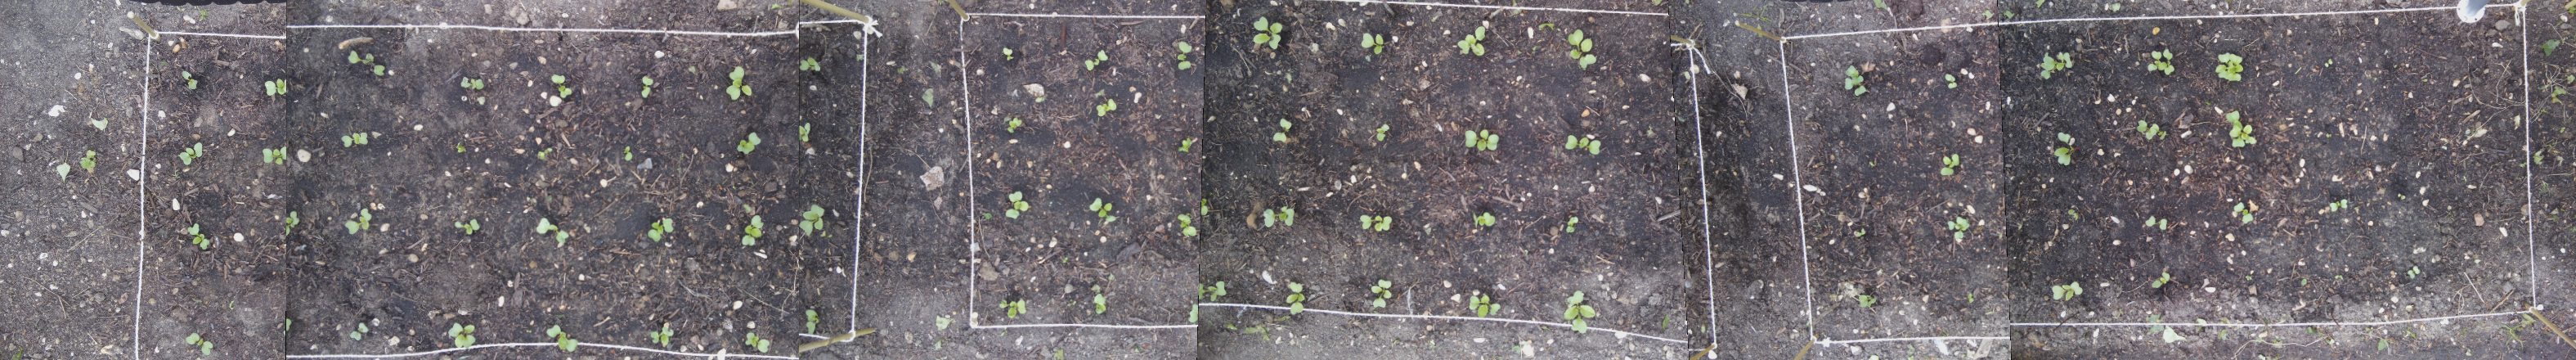
\includegraphics[width=\linewidth]{pics/cropbed.png}\\
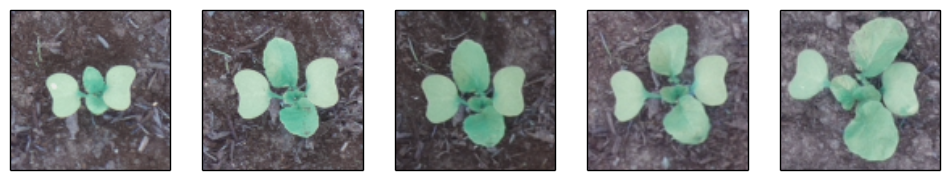
\includegraphics[width=\linewidth]{pics/growth.png}\\
\end{column}
\end{columns}

\end{frame}


\begin{frame}{Context: a robot...}%

\only<1>{
...for weeding...

\movie[label=mavideo,width=10cm,showcontrols,autostart]{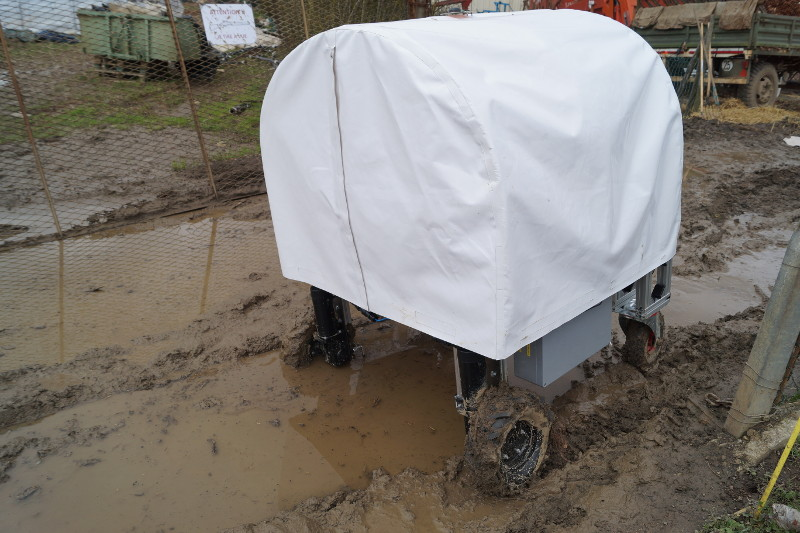
\includegraphics[width=.8\linewidth]{pics/lthink}}{weeding.mp4}\\%
}

\only<2-3>{
...for monitoring the growth of plants.

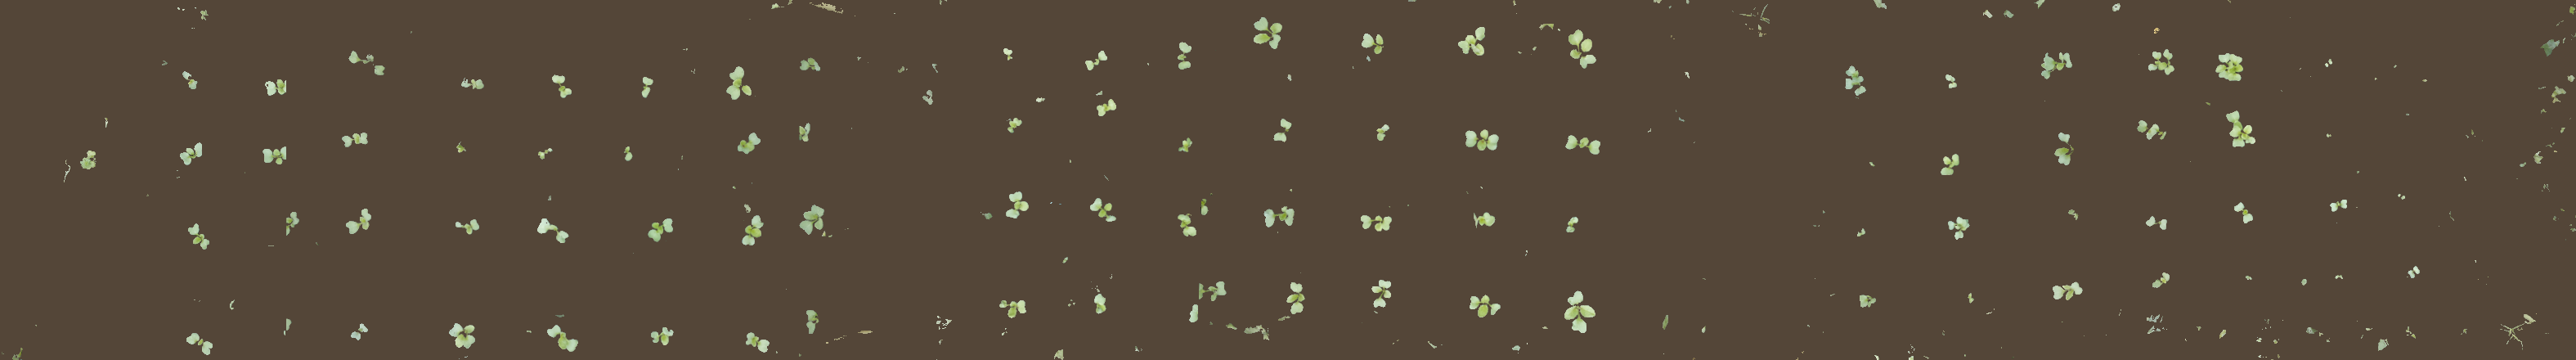
\includegraphics[width=\linewidth]{pics/cropbed_style2}\\

\movie[label=mavideo,width=4cm,showcontrols,autostart]{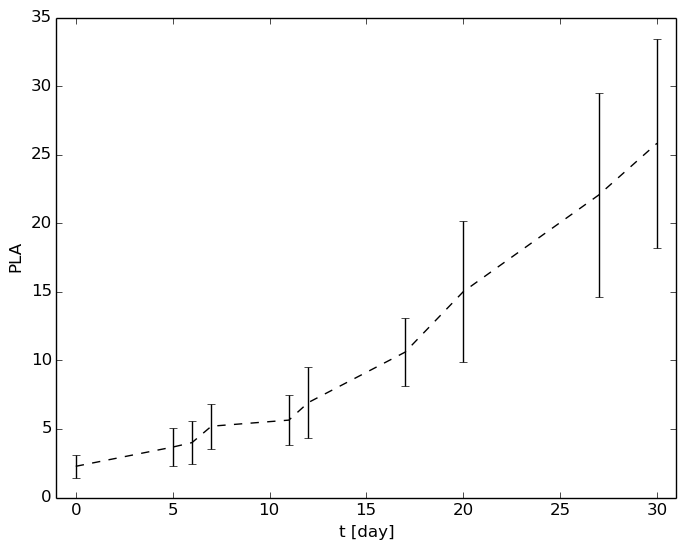
\includegraphics[width=.35\linewidth]{pics/PLAstat}}{pics/growth.mp4}
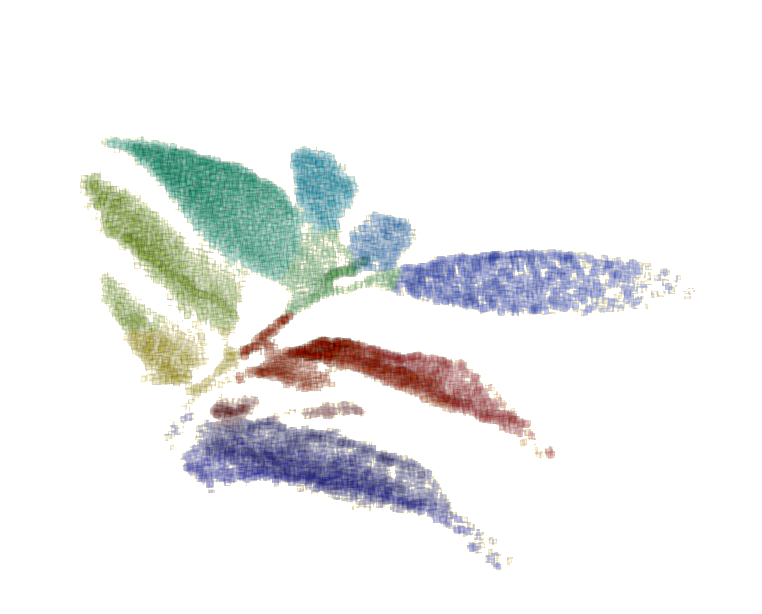
\includegraphics[width=.3\linewidth]{pics/seg_nobg}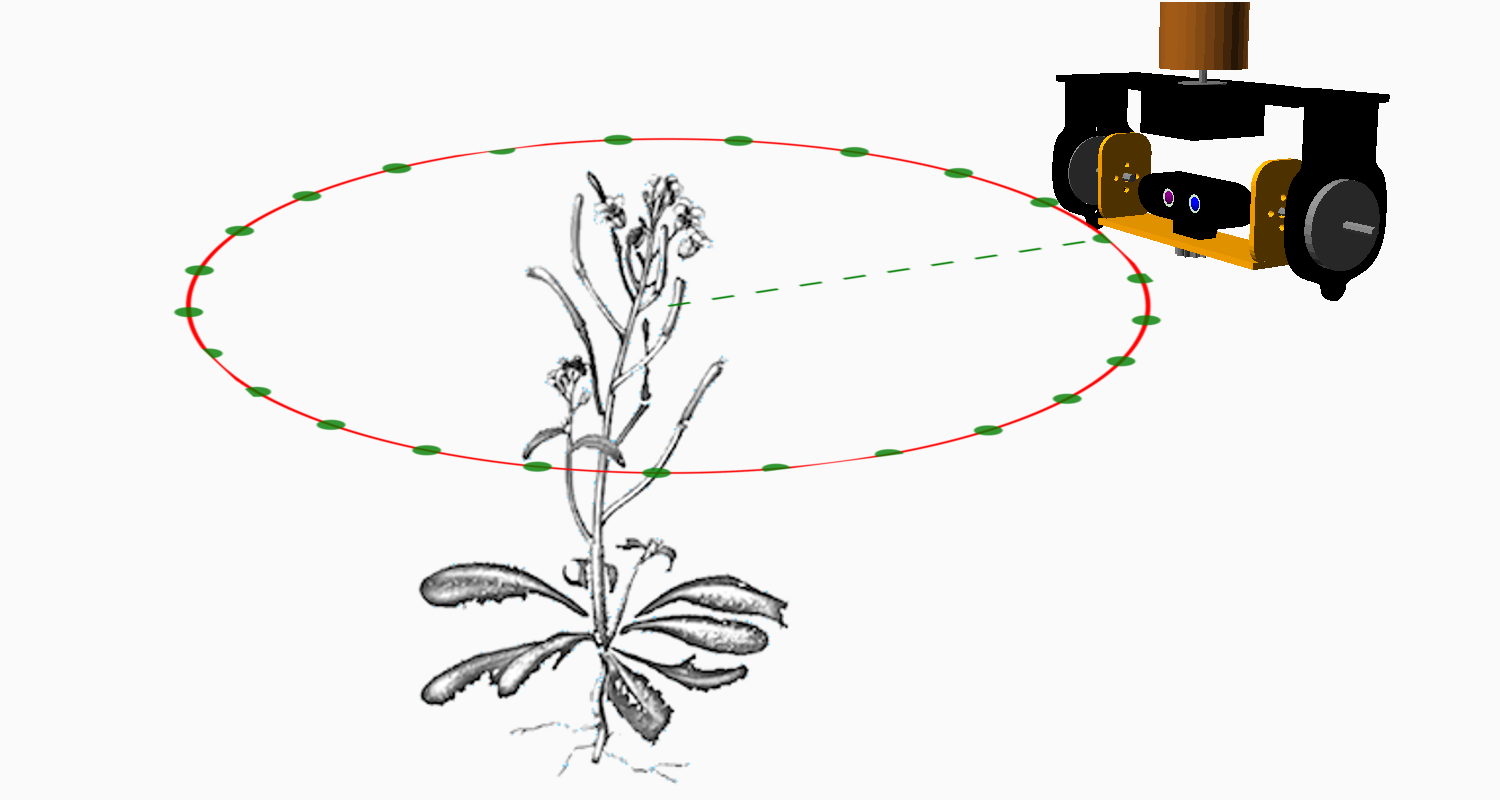
\includegraphics[width=.3\linewidth]{pics/scanner}\\
Growth dynamics
}

\only<2>{
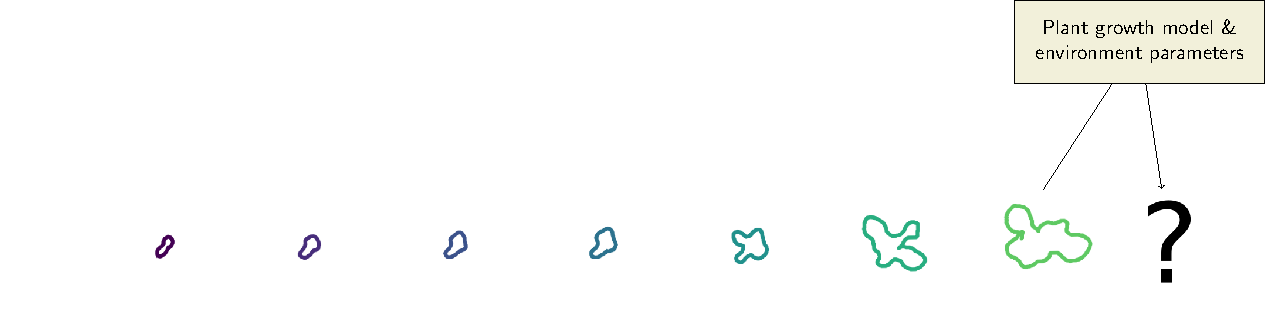
\includegraphics[width=\linewidth]{pics/trackSingle/guess.pdf}\\
}
\only<3>{
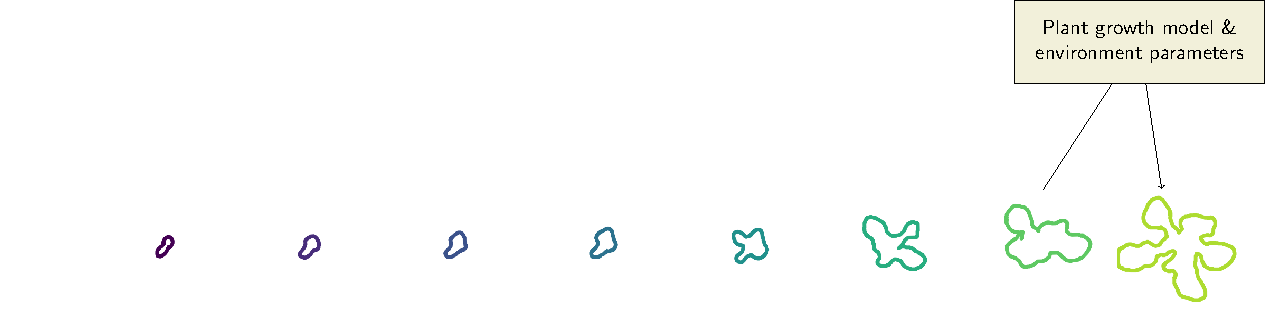
\includegraphics[width=\linewidth]{pics/trackSingle/pred0}\\
}

\end{frame}

\begin{frame}{Objectives of computer vision}%

\begin{columns}
\begin{column}{.5\linewidth}
\begin{itemize}
   \item<1-3> Segmentation
   \item<2-3> Mapping
   \item<3> Reconstruction (see also tomorrow)
\end{itemize}
\end{column}
\begin{column}{.5\linewidth}

\end{column}
\end{columns}

\end{frame}

